\paragraph{计算 Tucker 分解。} 与计算起来是 NP 难的 CP 分解不同，求出一个精确的 Tucker 分解（特别是具有最小多重线性秩的那个）可以在多项式时间内通过逐次 SVD 完成。 

Tucker 分解算法的基本思路，是在模 $n$ 上独立于其余各模，求出
$R_n$ 个主导的左奇异向量。该算法称为 \textit{高阶奇异值分解（Higher-Order SVD, HOSVD）}~\citep{de2000multilinear}，其流程画在下面。 为简单起见，我们以 $N=4$ 为例演示这一过程：
\begin{align*}
    &\begin{tikzpicture}[baseline=\baseline]
    \tikzset{tensor/.style = {minimum size = 0.5cm,shape = circle,thick,draw=black,inner sep = 0pt}, edge/.style = {thick,line width=.4mm},every loop/.style={}}
    \def\x{0}
    \def\y{0}
    \node[tensor,fill=green!50!red!50!white] (A) at (\x-5.5,\y){\scalebox{0.85}{$\Tt$}};
    \draw[edge] (A) -- (\x-5.5,\y+0.75) node [midway,left]
    {\scalebox{0.7}{\dimcolor{$d_1$}}};
    \draw[edge] (A) -- (\x-5.5,\y-0.75) node [midway,left]
    {\scalebox{0.7}{\dimcolor{$d_3$}}};
    \draw[edge] (\x-5.75,\y+0.05) -- (\x-6.2,\y-0.3) node [midway,above]
    {\scalebox{0.7}{\dimcolor{$d_2$}}};
    \draw[edge] (\x-5.25,\y+0.05) -- (\x-4.7,\y-0.3) node [midway,above]
    {\scalebox{0.7}{\dimcolor{$d_4$}}};
    \node[draw=none] at (\x-3,\y){$\underrightarrow{\text{mode-1 matricization}}$};
    \node[tensor,fill=green!50!red!50!white] (A) at (\x-0.5,\y){\scalebox{0.85}{$\Tb$}};
    \draw[edge] (\x-0.35,\y+0.2) -- (\x,\y+0.2) --(\x,\y+0.1) -- (\x
    +0.35,\y+0.1) node [midway,above]
    {\scalebox{0.7}{\dimcolor{$d_2$}}};
    \draw[edge] (\x-0.35,\y-0.2) -- (\x,\y-0.2) -- (\x,\y-0.1) -- (\x+0.35,\y-0.1) node [midway,below]
    {\scalebox{0.7}{\dimcolor{$d_4$}}};
     \draw[edge] (A) -- (\x+0.35,\y)node [right]
    {\scalebox{0.7}{\dimcolor{$d_3$}}};
     \draw[edge] (A) -- (\x-1.25,\y) node [midway,above]
    {\scalebox{0.7}{\dimcolor{$d_1$}}};
    \node[draw=none] at (\x+1,\y){$\rightarrow$};
    \node[tensor, path picture={
    \fill[fill=blue!50!white](path picture bounding box.south east)
        -- 
    (path picture bounding box.north west) --
    (path picture bounding box.north east) -- cycle;
    }, shift={(\x+1.5,\y)}] (U_1) {\scalebox{0.8}{$\Ub_1$}};
    \node[tensor,fill=red!50!white] (Sigma_1) at (\x+2.5,\y){\scalebox{0.85}{$\Sigmab_1$}};
    \node[tensor, path picture={
    \fill[fill=red!60!white](path picture bounding box.south west)
        -- 
    (path picture bounding box.north east) --
    (path picture bounding box.north west) -- cycle;
    }, shift={(\x+3.5,\y)}] (V_1) {\scalebox{0.8}{$\Vb_1$}};
    \draw[edge](V_1) -- (\x+4.5,\y) node [right]{\scalebox{0.7}{\textcolor{gray}{$d_3$}}};
    \draw[edge] (U_1) -- (Sigma_1)node [midway,above]
    {\scalebox{0.7}{\dimcolor{$R_1$}}};
    \draw[edge] (U_1) -- (\x+1.5,\y-0.7)node [midway,left]
    {\scalebox{0.7}{\dimcolor{$d_1$}}};
    \draw[edge] (Sigma_1) -- (V_1) node[midway,above]    {\scalebox{0.7}{\dimcolor{$R_1$}}};
    \draw[edge] (\x+3.7,\y+0.15) -- (\x+4,\y+0.15) --(\x+4,\y+0.1) -- (\x+4.5,\y+0.1) node [midway,above]
    {\scalebox{0.7}{\dimcolor{$d_2$}}};
    \draw[edge] (\x+3.65,\y-0.2) -- (\x+4,\y-0.2) -- (\x+4,\y-0.1) -- (\x+4.5,\y-0.1) node [midway,below]
    {\scalebox{0.7}{\dimcolor{$d_4$}}};
    \node[draw=none] at (\x+5.75,\y){\text{Keep $\Ub_1$}.};
\end{tikzpicture}\\
&\begin{tikzpicture}[baseline=\baseline]
    \tikzset{tensor/.style = {minimum size = 0.5cm,shape = circle,thick,draw=black,inner sep = 0pt}, edge/.style = {thick,line width=.4mm},every loop/.style={}}
    \def\y{0}
    \def\x{0}
    \node[tensor,fill=green!50!red!50!white] (A) at (\x-2.5,\y){\scalebox{0.85}{$\Tt$}};
    \draw[edge] (A) -- (\x-2.5,\y+0.75) node [midway,left]
    {\scalebox{0.7}{\dimcolor{$d_1$}}};
    \draw[edge] (A) -- (\x-2.5,\y-0.75) node [midway,left]
    {\scalebox{0.7}{\dimcolor{$d_3$}}};
    \draw[edge] (\x-2.75,\y+0.05) -- (\x-3.2,\y-0.3) node [midway,above]
    {\scalebox{0.7}{\dimcolor{$d_2$}}};
    \draw[edge] (\x-2.25,\y+0.05) -- (\x-1.7,\y-0.3) node [midway,above]
    {\scalebox{0.7}{\dimcolor{$d_4$}}};
    \node[draw=none] at (\x,\y){$\underrightarrow{\text{mode-2 matricization}}$};
    \node[tensor,fill=green!50!red!50!white] (A) at (\x+2.5,\y){\scalebox{0.85}{$\Tb$}};
    \draw[edge] (A) -- (\x+1.75,\y) node [midway,above]
    {\scalebox{0.7}{\dimcolor{$d_2$}}};
    \draw[edge] (A) -- (\x+3.35,\y)node [right]
    {\scalebox{0.7}{\dimcolor{$d_3$}}};
    \draw[edge] (\x+2.65,\y+0.2) -- (\x+3,\y+0.2) -- (\x+3,\y+0.1) -- (\x+3.35,\y+0.1)node [midway,above]
    {\scalebox{0.7}{\dimcolor{$d_1$}}};
    \draw[edge] (\x+2.65,\y-0.2) -- (\x+3,\y-0.2) -- (\x+3,\y-0.1) -- (\x+3.35,\y-0.1)node [midway,below]
    {\scalebox{0.7}{\dimcolor{$d_4$}}};
    \node[draw=none] at (\x+4,\y){$\rightarrow$};
    \node[tensor, path picture={
    \fill[fill=blue!40!white](path picture bounding box.south east)
        -- 
    (path picture bounding box.north west) --
    (path picture bounding box.north east) -- cycle;
    }, shift={(\x+4.5,\y)}] (U_2) {\scalebox{0.8}{$\Ub_2$}};
    \node[tensor,fill=red!40!white] (Sigma_2) at (\x+5.5,\y){\scalebox{0.85}{$\Sigmab_2$}};
    \node[tensor, path picture={
    \fill[fill=red!50!white](path picture bounding box.south west)
        -- 
    (path picture bounding box.north east) --
    (path picture bounding box.north west) -- cycle;
    }, shift={(\x+6.5,\y)}] (V_2) {\scalebox{0.8}{$\Vb_2$}};
    \draw[edge](V_2) -- (\x+7.5,\y) node [right]{\scalebox{0.7}{\dimcolor{$d_3$}}};
    \draw[edge] (U_2) -- (Sigma_2)node [midway,above]
    {\scalebox{0.7}{\dimcolor{$R_2$}}};
    \draw[edge] (U_2) -- (\x+4.5,\y-0.7)node [midway,left]
    {\scalebox{0.7}{\dimcolor{$d_2$}}};
    \draw[edge] (Sigma_2) -- (V_2) node[midway,above] {\scalebox{0.7}{\dimcolor{$R_2$}}};
    \draw[edge] (\x+6.71,\y+0.15) -- (\x+7,\y+0.15) --(\x+7,\y+0.1) -- (\x+7.5,\y+0.1) node [midway,above]
    {\scalebox{0.7}{\dimcolor{$d_1$}}};
    \draw[edge] (\x+6.65,\y-0.2) -- (\x+7,\y-0.2) -- (\x+7,\y-0.1) -- (\x+7.5,\y-0.1) node [midway,below]
    {\scalebox{0.7}{\dimcolor{$d_4$}}};
    \node[draw=none] at (\x+8.75,\y){\text{Keep $\Ub_2$}.};
\end{tikzpicture}\\
&\begin{tikzpicture}[baseline=\baseline]
    \tikzset{tensor/.style = {minimum size = 0.5cm,shape = circle,thick,draw=black,inner sep = 0pt}, edge/.style = {thick,line width=.4mm},every loop/.style={}}
    \def\y{0}
    \def\x{0}
    \node[tensor,fill=green!50!red!50!white] (A) at (\x-2.5,\y){\scalebox{0.85}{$\Tt$}};
    \draw[edge] (A) -- (\x-2.5,\y+0.75) node [midway,left]
    {\scalebox{0.7}{\dimcolor{$d_1$}}};
    \draw[edge] (A) -- (\x-2.5,\y-0.75) node [midway,left]
    {\scalebox{0.7}{\dimcolor{$d_3$}}};
    \draw[edge] (\x-2.75,\y+0.05) -- (\x-3.2,\y-0.3) node [midway,above]
    {\scalebox{0.7}{\dimcolor{$d_2$}}};
    \draw[edge] (\x-2.25,\y+0.05) -- (\x-1.7,\y-0.3) node [midway,above]
    {\scalebox{0.7}{\dimcolor{$d_4$}}};
    \node[draw=none] at (\x,\y){$\underrightarrow{\text{mode-3 matricization}}$};
    \node[tensor,fill=green!50!red!50!white] (A) at (\x+2.5,\y){\scalebox{0.85}{$\Tb$}};
    \draw[edge] (A) -- (\x+1.75,\y) node [midway,above]
    {\scalebox{0.7}{\dimcolor{$d_3$}}};
    \draw[edge] (A) -- (\x+3.35,\y)node [right]
    {\scalebox{0.7}{\dimcolor{$d_2$}}};
    \draw[edge] (\x+2.65,\y+0.2) -- (\x+3,\y+0.2) -- (\x+3,\y+0.1) -- (\x+3.35,\y+0.1)node [midway,above]
    {\scalebox{0.7}{\dimcolor{$d_1$}}};
    \draw[edge] (\x+2.65,\y-0.2) -- (\x+3,\y-0.2) -- (\x+3,\y-0.1) -- (\x+3.35,\y-0.1)node [midway,below]
    {\scalebox{0.7}{\dimcolor{$d_4$}}};
    \node[draw=none] at (\x+4,\y){$\rightarrow$};
    \node[tensor, path picture={
    \fill[fill=blue!30!white](path picture bounding box.south east)
        -- 
    (path picture bounding box.north west) --
    (path picture bounding box.north east) -- cycle;
    }, shift={(\x+4.5,\y)}] (U_3) {\scalebox{0.8}{$\Ub_3$}};
    \node[tensor,fill=red!30!white] (Sigma_3) at (\x+5.5,\y){\scalebox{0.85}{$\Sigmab_3$}};
    \node[tensor, path picture={
    \fill[fill=red!40!white](path picture bounding box.south west)
        -- 
    (path picture bounding box.north east) --
    (path picture bounding box.north west) -- cycle;
    }, shift={(\x+6.5,\y)}] (V_3) {\scalebox{0.8}{$\Vb_3$}};
    \draw[edge](V_3) -- (\x+7.5,\y) node [right]{\scalebox{0.7}{\dimcolor{$d_2$}}};
    \draw[edge] (U_3) -- (Sigma_3)node [midway,above]
    {\scalebox{0.7}{\dimcolor{$R_3$}}};
    \draw[edge] (U_3) -- (\x+4.5,\y-0.7)node [midway,left]
    {\scalebox{0.7}{\dimcolor{$d_3$}}};
    \draw[edge] (Sigma_3) -- (V_3) node[midway,above] {\scalebox{0.7}{\dimcolor{$R_3$}}};
    \draw[edge] (\x+6.71,\y+0.15) -- (\x+7,\y+0.15) --(\x+7,\y+0.1) -- (\x+7.5,\y+0.1) node [midway,above]
    {\scalebox{0.7}{\dimcolor{$d_1$}}};
    \draw[edge] (\x+6.65,\y-0.2) -- (\x+7,\y-0.2) -- (\x+7,\y-0.1) -- (\x+7.5,\y-0.1) node [midway,below]
    {\scalebox{0.7}{\dimcolor{$d_4$}}};
    \node[draw=none] at (\x+8.75,\y){\text{Keep $\Ub_3$.}};
\end{tikzpicture}\\
&\begin{tikzpicture}[baseline=\baseline]
    \tikzset{tensor/.style = {minimum size = 0.5cm,shape = circle,thick,draw=black,inner sep = 0pt}, edge/.style = {thick,line width=.4mm},every loop/.style={}}
    \def\y{0}
    \def\x{0}
    \node[tensor,fill=green!50!red!50!white] (A) at (\x-2.5,\y){\scalebox{0.85}{$\Tt$}};
    \draw[edge] (A) -- (\x-2.5,\y+0.75) node [midway,left]
    {\scalebox{0.7}{\dimcolor{$d_1$}}};
    \draw[edge] (A) -- (\x-2.5,\y-0.75) node [midway,left]
    {\scalebox{0.7}{\dimcolor{$d_3$}}};
    \draw[edge] (\x-2.75,\y+0.05) -- (\x-3.2,\y-0.3) node [midway,above]
    {\scalebox{0.7}{\dimcolor{$d_2$}}};
    \draw[edge] (\x-2.25,\y+0.05) -- (\x-1.7,\y-0.3) node [midway,above]
    {\scalebox{0.7}{\dimcolor{$d_4$}}};
    \node[draw=none] at (\x,\y){$\underrightarrow{\text{mode-4 matricization}}$};
    \node[tensor,fill=green!50!red!50!white] (A) at (\x+2.5,\y){\scalebox{0.85}{$\Tb$}};
    \draw[edge] (A) -- (\x+1.75,\y) node [midway,above]
    {\scalebox{0.7}{\dimcolor{$d_4$}}};
    \draw[edge] (A) -- (\x+3.35,\y)node [right]
    {\scalebox{0.7}{\dimcolor{$d_2$}}};
    \draw[edge] (\x+2.65,\y+0.2) -- (\x+3,\y+0.2) -- (\x+3,\y+0.1) -- (\x+3.35,\y+0.1)node [midway,above]
    {\scalebox{0.7}{\dimcolor{$d_1$}}};
    \draw[edge] (\x+2.65,\y-0.2) -- (\x+3,\y-0.2) -- (\x+3,\y-0.1) -- (\x+3.35,\y-0.1)node [midway,below]
    {\scalebox{0.7}{\dimcolor{$d_3$}}};
    \node[draw=none] at (\x+4,\y){$\rightarrow$};
    \node[tensor, path picture={
    \fill[fill=blue!20!white](path picture bounding box.south east)
        -- 
    (path picture bounding box.north west) --
    (path picture bounding box.north east) -- cycle;
    }, shift={(\x+4.5,\y)}] (U_4) {\scalebox{0.8}{$\Ub_4$}};
    \node[tensor,fill=red!20!white] (Sigma_4) at (\x+5.5,\y){\scalebox{0.85}{$\Sigmab_4$}};
    \node[tensor, path picture={
    \fill[fill=red!30!white](path picture bounding box.south west)
        -- 
    (path picture bounding box.north east) --
    (path picture bounding box.north west) -- cycle;
    }, shift={(\x+6.5,\y)}] (V_4) {\scalebox{0.8}{$\Vb_4$}};
    \draw[edge](V_4) -- (\x+7.5,\y) node [right]{\scalebox{0.7}{\dimcolor{$d_2$}}};
    \draw[edge] (U_4) -- (Sigma_4)node [midway,above]
    {\scalebox{0.7}{\dimcolor{$R_4$}}};
    \draw[edge] (U_4) -- (\x+4.5,\y-0.7)node [midway,left]
    {\scalebox{0.7}{\dimcolor{$d_4$}}};
    \draw[edge] (Sigma_4) -- (V_4) node[midway,above] {\scalebox{0.7}{\dimcolor{$R_4$}}};
    \draw[edge] (\x+6.71,\y+0.15) -- (\x+7,\y+0.15) --(\x+7,\y+0.1) -- (\x+7.5,\y+0.1) node [midway,above]
    {\scalebox{0.7}{\dimcolor{$d_1$}}};
    \draw[edge] (\x+6.65,\y-0.2) -- (\x+7,\y-0.2) -- (\x+7,\y-0.1) -- (\x+7.5,\y-0.1) node [midway,below]
    {\scalebox{0.7}{\dimcolor{$d_3$}}};
    \node[draw=none] at (\x+8.75,\y){\text{Keep $\Ub_4$.}};
\end{tikzpicture}
\end{align*}
若上述所有 SVD 都是精确的，即对每个 $n$ 有 $R_n = \rank(\Tt_{(n)})$，则对所有 $n$ 均有 $\Tt \times_n \Ub_n\Ub_n^\ts = \Tt$，从而 $\Tt = \Tt\times_1\Ub_1\Ub_1^\ts\times_2\cdots\times_N\Ub_N\Ub_N^\ts$。举例来说，当 $N=4$ 时有：
$$
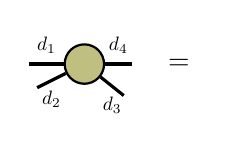
\begin{tikzpicture}[baseline=-0.5ex]
    \tikzset{tensor/.style = {minimum size = 0.5cm,shape = circle,thick,draw=black,inner sep = 0pt}, edge/.style = {thick,line width=.4mm},every loop/.style={}}
    \def\x{6}
    \def\y{0}   \node[tensor,fill=green!50!red!50!white] (T) at (\x+1,\y) {$\Tt$};
    \draw[edge] (T) -- (\x+0.3,0) node [midway,above] {\scalebox{0.7}{\dimcolor{$d_1$}}};
    \draw[edge] (T) -- (\x+1.6,0) node [midway,above] {\scalebox{0.7}{\dimcolor{$d_4$}}};;
    \draw[edge] (T) -- (\x+0.4,-0.3) node [midway, below] {\scalebox{0.7}{\dimcolor{$d_2$}}};
    \draw[edge] (T) -- (\x+1.5,-0.4)node [midway, below] {\scalebox{0.7}{\dimcolor{$d_3$}}};
    \node[draw = none] at (\x+2.2,0){$=$};
\end{tikzpicture}
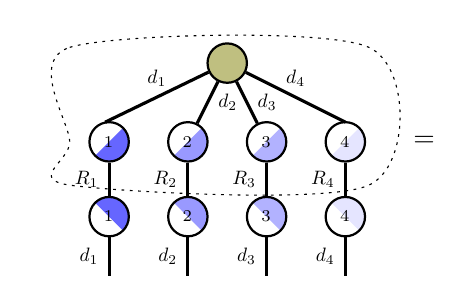
\begin{tikzpicture}[baseline=-0.5ex]
    \tikzset{tensor/.style = {minimum size = 0.5cm,shape = circle,thick,draw=black,inner sep = 0pt}, edge/.style = {thick,line width=.4mm},every loop/.style={}}
    \def\x{6}
    \def\y{0} 
    \node[tensor,fill=green!50!red!50!white] (T) at (\x+4.5,\y+1) {$\Tt$};
    \node[tensor, path picture={
    \fill[fill=blue!60!white](path picture bounding box.north east)
        -- 
    (path picture bounding box.south east) --
    (path picture bounding box.south west) -- cycle;
    }, shift={(\x+3,\y)}] (U_1) {\scalebox{0.85}{$\Ub_1$}};
    \node[tensor, path picture={
    \fill[fill=blue!60!white](path picture bounding box.south east)
        -- 
    (path picture bounding box.north east) --
    (path picture bounding box.north west) -- cycle;
    }, shift={(\x+3,\y-0.95)}] (Ut_1) {\scalebox{0.85}{$\Ub_1$}};
    \node[tensor, path picture={
    \fill[fill=blue!40!white](path picture bounding box.north east)
        -- 
    (path picture bounding box.south east) --
    (path picture bounding box.south west) -- cycle;
    }, shift={(\x+4,\y)}] (U_2) {\scalebox{0.85}{$\Ub_2$}};
    \node[tensor, path picture={
    \fill[fill=blue!40!white](path picture bounding box.south east)
        -- 
    (path picture bounding box.north east) --
    (path picture bounding box.north west) -- cycle;
    }, shift={(\x+4,\y-0.95)}] (Ut_2) {\scalebox{0.85}{$\Ub_2$}};
    \node[tensor, path picture={
    \fill[fill=blue!30!white](path picture bounding box.north east)
    -- 
    (path picture bounding box.south west) --
    (path picture bounding box.south east) -- cycle;
    }, shift={(\x+5,\y)}] (U_3) {\scalebox{0.85}{$\Ub_3$}};
    \node[tensor, path picture={
    \fill[fill=blue!30!white](path picture bounding box.south east)
        -- 
    (path picture bounding box.north east) --
    (path picture bounding box.north west) -- cycle;
    }, shift={(\x+5,\y-0.95)}] (Ut_3) {\scalebox{0.85}{$\Ub_3$}};
    \node[tensor, path picture={
    \fill[fill=blue!10!white](path picture bounding box.north east)
    -- 
    (path picture bounding box.south west) --
    (path picture bounding box.south east) -- cycle;
    }, shift={(\x+6,\y)}] (U_4) {\scalebox{0.85}{$\Ub_4$}};
    \node[tensor, path picture={
    \fill[fill=blue!10!white](path picture bounding box.south east)
        -- 
    (path picture bounding box.north east) --
    (path picture bounding box.north west) -- cycle;
    }, shift={(\x+6,\y-0.95)}] (Ut_4) {\scalebox{0.85}{$\Ub_4$}};
    \draw[edge] (T) -- (\x+2.95,\y+0.25) node [midway, above] {\scalebox{0.7}{\dimcolor{$d_1$}}};
    \draw[edge] (T) -- (U_2) node [midway, right] {\scalebox{0.7}{\dimcolor{$d_2$}}};
    \draw[edge] (T) -- (U_3) node [midway, right] {\scalebox{0.7}{\dimcolor{$d_3$}}};
    \draw[edge] (T) -- (\x+6,\y+0.25) node [midway, above] {\scalebox{0.7}{\dimcolor{$d_4$}}};
    \draw[edge] (U_1) -- (\x+3,\y-0.7) node [midway, left] {\scalebox{0.7}{\dimcolor{$R_1$}}};
    \draw[edge] (U_2) -- (\x+4,\y-0.7) node [midway, left] {\scalebox{0.7}{\dimcolor{$R_2$}}};
    \draw[edge] (U_3) -- (\x+5,\y-0.7) node [midway, left] {\scalebox{0.7}{\dimcolor{$R_3$}}};
    \draw[edge] (U_4) -- (\x+6,\y-0.7) node [midway, left] {\scalebox{0.7}{\dimcolor{$R_4$}}};
    \draw[edge] (Ut_1) -- (\x+3,\y-1.7) node [midway, left] {\scalebox{0.7}{\dimcolor{$d_1$}}};
    \draw[edge] (Ut_2) -- (\x+4,\y-1.7) node [midway, left] {\scalebox{0.7}{\dimcolor{$d_2$}}};
    \draw[edge] (Ut_3) -- (\x+5,\y-1.7) node [midway, left] {\scalebox{0.7}{\dimcolor{$d_3$}}};
    \draw[edge] (Ut_4) -- (\x+6,\y-1.7) node [midway, left] {\scalebox{0.7}{\dimcolor{$d_4$}}};
    \draw[dash pattern=on 1pt off 2pt] plot[smooth cycle] coordinates { 
    (\x+2.5,\y) 
    (\x+2.5, \y+1.2) (\x+6.3,\y+1.2) (\x+6.3, \y-0.55)  (\x+2.5,\y-0.55)};
    \node[draw = none] at (\x+7,0){$=$};
\end{tikzpicture}
